\documentclass[12pt]{article}
\usepackage[a4paper, total={5.5in, 9in}]{geometry}
\usepackage{amsmath} % For mathematical formatting
\usepackage{changepage}
\usepackage[most]{tcolorbox}
\usepackage{textcomp} % for writing degrees
\usepackage{tikz} % For drawing the triangle
\usepackage{pgfplots}
\pgfplotsset{compat=1.18}
\usepackage{hyperref}

\title{Precalculus Worksheet 6.2}
\author{PCL Learning Center}
\date{}

\begin{document}
\maketitle

\begin{center}
    \textit{note: This worksheet may be used for two sessions, and\\no electronic devices may be used on this worksheet.}
\end{center}

\section*{Problem Set 1\\Difficulty level: Normal}
\subsection*{Problem 1}
Give the equation of an asymptote for the graph of \(f(x)=\tan(2x)\) on the interval \((0,\pi)\).

\subsection*{Problem 2}
Which of the following numbers are not in the domain of \(\tan(x)\).
\[\dfrac{3\pi}{2}, \hspace{0.2cm} 0, \hspace{0.2cm} \dfrac{\pi}{2}, \hspace{0.2cm}-\pi, \hspace{0.2cm}, \pi\]

\subsection*{Problem 3}
Which of the following numbers are not in the domain of \(\cot(x)\)?
\[
3\pi,\hspace{0.2cm}-\dfrac{\pi}{2},\hspace{0.2cm}\dfrac{\pi}{6},\hspace{0.2cm}\dfrac{3\pi}{4},\hspace{0.2cm}-\pi
\]

\subsection*{Problem 4}
Give the equations of the asymptotes for the graph of \(f(x) = \cot(x)\) on the interval \((\pi, 3\pi]\).

\subsection*{Problem 5}
Which of the following numbers are not in the domain of \(\csc(x)\)?
\[
-\dfrac{\pi}{4},\hspace{0.2cm}-\dfrac{\pi}{2},\hspace{0.2cm}-\dfrac{3\pi}{4},\hspace{0.2cm}-\pi,\hspace{0.2cm}0
\]

\subsection*{Problem 6}
On the domain of \([ -2\pi, 0 )\), for what value(s) of \(x\) will \(\sin(-x) = \csc(-x)\)?

\subsection*{Problem 7}
On the graph of \(f(x) = \sec(x)\) and the interval \((-2\pi, 2\pi)\), for what value(s) of \(x\) does \(f(x) = -1\)?

\subsection*{Problem 8}
Which of the following numbers are not in the domain of \(\sec(x)\)?
\[
0,\hspace{0.2cm}\dfrac{9\pi}{2},\hspace{0.2cm}9\pi,\hspace{0.2cm}\dfrac{7\pi}{2},\hspace{0.2cm}7\pi
\]

\section*{Problem Set 2\\Difficulty level: Hard}
\subsection*{Problem 1}
Sketch the graph of the function \(f(x)=\pi \tan(\pi x - \pi)-\pi\).
\subsection*{Problem 2}
Why are there no \(x-\)intercepts on the function \(f(x)=\csc(x)\)?

\newpage
\section*{Solutions for Set 1}
\subsection*{Problem 1}
\(x=\dfrac{\pi}{4},\hspace{0.2cm} x=\dfrac{3\pi}{4}\)
\subsection*{Problem 2}
\(\dfrac{3\pi}{2}, \hspace{0.2cm} \dfrac{\pi}{2}\)
\subsection*{Problem 3}
\(3\pi, \hspace{0.2cm} -\pi\)
\subsection*{Problem 4}
\(x=2\pi, \hspace{0.2cm} x=3\pi\)
\subsection*{Problem 5}
\(-\pi, \hspace{0.2cm} 0\)
\subsection*{Problem 6}
\(x=-\dfrac{3\pi}{2}, \hspace{0.2cm} x=-\dfrac{\pi}{2}\)
\subsection*{Problem 7}
\(x=-\pi, \hspace{0.2cm} x=\pi\)
\subsection*{Problem 8}
\(\dfrac{9\pi}{2},\hspace{0.2cm} \dfrac{7\pi}{2}\)

\section*{Solutions for Set 2}
\subsection*{Problem 1}
\begin{center}
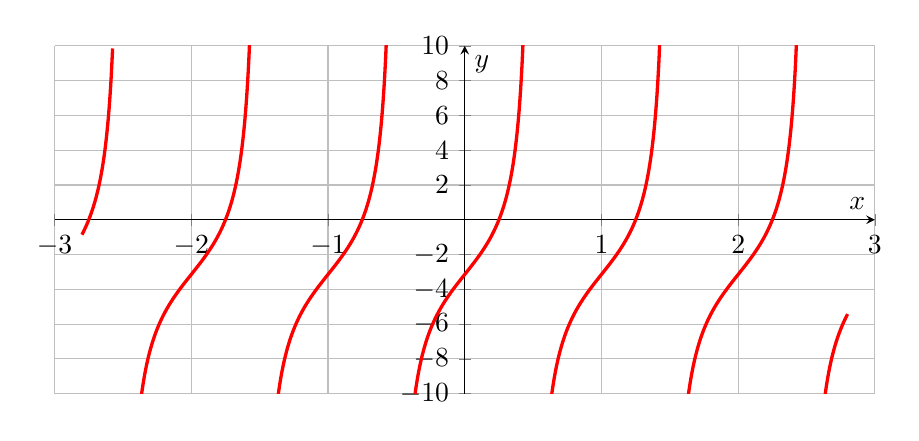
\begin{tikzpicture}
\begin{axis}[
    axis lines=middle,
    width=12cm,  % Ancho aumentado
    height=6cm,  % Altura reducida
    xmin=-3, xmax=3,  % Rango x reducido
    ymin=-10, ymax=10,  % Rango y ampliado
    xtick={-3,-2,...,3},
    ytick={-10,-8,...,10},
    grid=both,
    xlabel=\(x\),
    ylabel=\(y\),
    restrict y to domain=-12:12,  % Limita el rango y para evitar líneas largas
    unbounded coords=jump  % Omite puntos cerca de las asíntotas
]
\addplot[domain=-2.8:2.8, samples=500, very thick, red, smooth] {pi*tan(deg(pi*x - pi)) - pi};
\end{axis}
\end{tikzpicture}
\end{center}

For a more detailed graph, sketch \(f(x)=\pi \tan(\pi x - \pi)-\pi\) on \href{https://www.desmos.com/calculator}{Desmos} or \href{https://www.geogebra.org/graphing?lang=en}{GeoGebra} to see the solution.

\subsection*{Problem 2}
Because \(\csc(x)\) is undefined at \(x=0\), since \(\csc(x)=\dfrac{1}{\sin(x)}\) for all real numbers, except where \(\sin(x)=0\).


\end{document}
